\documentclass[tikz, border=10pt]{standalone}
\usetikzlibrary{shapes.geometric, arrows.meta, positioning}

\begin{document}
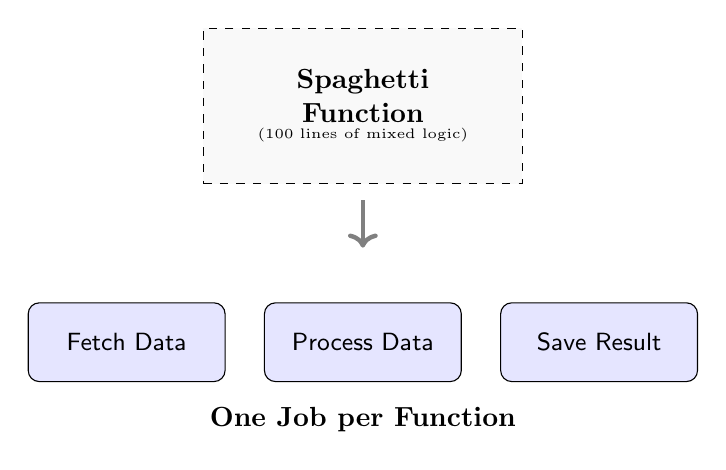
\begin{tikzpicture}[
    box/.style={rectangle, draw, minimum width=2.5cm, minimum height=1cm, rounded corners, fill=blue!10, font=\sffamily\small}
]

% Big Function
\node[draw, dashed, inner sep=15pt, fill=gray!5] (big) at (0,3) {
    \begin{minipage}{3cm}
    \centering \textbf{Spaghetti Function}\\ \tiny (100 lines of mixed logic)
    \end{minipage}
};

% Split arrows
\draw[ultra thick, ->, gray] (0, 1.8) -- (0, 1.2);

% Small functions
\node[box] (fetch) at (-3, 0) {Fetch Data};
\node[box] (process) at (0, 0) {Process Data};
\node[box] (save) at (3, 0) {Save Result};

\node[below=2mm of process] {\textbf{One Job per Function}};

\end{tikzpicture}
\end{document}
